\documentclass[aspectratio=169,
hyperref={colorlinks,urlcolor=blue}
]{beamer}


%\usetheme{Pittsburgh}
\usetheme{default}
\usepackage{colortbl}%colored tables
%For using helvetica font:
\usepackage[scaled]{helvet}
\usepackage[T1]{fontenc}
\renewcommand\familydefault{\sfdefault}
\urlstyle{same} %sets the fonts for urls
\usepackage{pdfpages}
\usepackage{siunitx}
\usepackage{caption}
\usepackage{pifont}%for dings
\usepackage{pgfplots}%for 3d plotting
\pgfplotsset{compat = newest}
\usepackage{mathtools}%box in align env \Aboxed
\usepackage[american,smartlabels]{circuitikz}%for drawing circuits
\usepackage{multimedia}
\usepackage{animate}
\usepackage{xcolor}


\usetikzlibrary{arrows}
\usetikzlibrary {3d} 
\usetikzlibrary{decorations.markings, math}
\usetikzlibrary{intersections, pgfplots.fillbetween}
\usetikzlibrary {shapes.geometric} 


%\definecolor{myblue}{RGB}{5, 34, 150}
\definecolor{myblue2}{RGB}{5, 34, 150}
\definecolor{myblue}{RGB}{0,36,82}
\definecolor{myred}{RGB}{207, 2, 13}
\definecolor{mygreen}{RGB}{0, 158, 11}
\definecolor{myyellow}{RGB}{220,220,0}
\definecolor{qblue}{RGB}{0,36,82}
\definecolor{qgold}{RGB}{250,189,15}
\definecolor{qred}{RGB}{185,14,49}
\definecolor{cblue}{rgb}{0.13, 0.67, 0.8}
\definecolor{corange}{rgb}{0.8, 0.34, 0.0}
\definecolor{cpurple}{rgb}{0.54, 0.29, 0.42}

%%%%%%%%%%%% General settings
\setbeamercolor{frametitle}{fg=black}
\setbeamercolor{title}{fg=black}
\setbeamercolor{author}{fg=myblue2}

\beamertemplatenavigationsymbolsempty %no navigation controls at bottom of slides
%\setbeamertemplate{footline}[frame number]
\usefonttheme{professionalfonts} 
\setbeamerfont{title}{series=\bfseries,parent=structure}
\setbeamerfont{frametitle}{series=\bfseries,parent=structure}

%%%%%%%%%%%%Lists
\setbeamertemplate{itemize item}[circle] %{\color{myblue}$\circ$}
\setbeamertemplate{itemize subitem}{\color{myblue2}$\circ$}
\setbeamertemplate{itemize subsubitem}{\color{myblue2}$\cdot$}
\setbeamercolor{itemize item}{bg=myblue2,fg=myblue2}
\setbeamercolor{enumerate item}{bg=myblue2,fg=myblue2}
%%%%%%%%%%%%%%%%%%%%%%%%%%%%

%%%%%%%%%%%%Blocks
\setbeamertemplate{blocks}[rounded]
%Default block
\setbeamercolor{block title}{bg=myblue2, fg=white}
\setbeamercolor{block body}{bg=myblue2!10}
\setbeamerfont{block body}{size=\scriptsize}
\setbeamerfont{block title}{size=\scriptsize}
%Alert block
\setbeamercolor{block title alerted}{bg= myblue2, fg=white}
\setbeamercolor{block body alerted}{bg=myblue2!10}
\setbeamerfont{block body alerted}{size=\scriptsize}
\setbeamerfont{block title alerted}{size=\scriptsize}
%example block
\setbeamercolor{block title example}{bg=mygreen, fg=white}
\setbeamercolor{block body example}{bg=mygreen!10}
\setbeamerfont{block body example}{size=\scriptsize}
\setbeamerfont{block title example}{size=\scriptsize}
%%%%%%%%%%%%%%%%55


%%%%%%%%%%%%Figures and captions
\captionsetup{font=scriptsize,labelfont=scriptsize}
%\setbeamertemplate{caption}{\raggedright\insertcaption\par}
\newenvironment{capfig}[3]{\begin{figure}\includegraphics[width=#1\textwidth]{#2}\caption*{\textit{#3}}\end{figure}}{}

%\makeatother
%\setbeamertemplate{footline}
%{
%  \leavevmode%
%  \hbox{%
%  \begin{beamercolorbox}[wd=.4\paperwidth,ht=2.25ex,dp=1ex,center]{author in head/foot}%
%    \usebeamerfont{author in head/foot}\insertshortauthor
%  \end{beamercolorbox}%
%  \begin{beamercolorbox}[wd=.6\paperwidth,ht=2.25ex,dp=1ex,center]{title in head/foot}%
%    \usebeamerfont{title in head/foot}\insertshorttitle\hspace*{3em}
%    \insertframenumber{} / \inserttotalframenumber\hspace*{1ex}
%  \end{beamercolorbox}
%  }%
%  \vskip0pt%
%}
%\makeatletter

\makeatother
\setbeamertemplate{footline}
{
  \leavevmode%
  \hbox{%
\begin{beamercolorbox}[wd=.27\paperwidth,ht=2.25ex,dp=1ex,center]{author in head/foot}%
    \color{black}{\insertinstitute}
\end{beamercolorbox}
  \begin{beamercolorbox}[wd=.27\paperwidth,ht=2.25ex,dp=1ex,center]{author in head/foot}%
    \color{black}{\inserttitle}
  \end{beamercolorbox}%
  \begin{beamercolorbox}[wd=.27\paperwidth,ht=2.25ex,dp=1ex,center]{title in head/foot}%
    \color{black}{\insertshortauthor}
  \end{beamercolorbox}
  \begin{beamercolorbox}[wd=.27\paperwidth,ht=2.25ex,dp=1ex,center]{title in head/foot}%
    \hspace{.28\paperwidth}\color{black} \insertframenumber{} / \inserttotalframenumber\hspace*{1ex}
  \end{beamercolorbox}
  }%
  \vskip0pt%
}
\makeatletter

\setbeamertemplate{title page}
{
  \begin{tikzpicture}[remember picture,overlay]
    \def\barh{4}%15
  
    \draw[color=myblue2,line width=\barh] ([yshift=-0.5*\barh]current page.north west) -- ([yshift=-0.5*\barh,xshift=-0.67\paperwidth]current page.north east);
    \draw[color=myblue2,line width=\barh] ([yshift=-0.5*\barh,xshift=-0.67\paperwidth]current page.north east) -- ([yshift=-0.5*\barh,xshift=-0.34\paperwidth]current page.north east);
    \draw[color=myblue2,line width=\barh] ([yshift=-0.5*\barh,xshift=-0.34\paperwidth]current page.north east) -- ([yshift=-0.5*\barh]current page.north east); 
  
    \draw[color=myblue2,line width=\barh] ([yshift=0.5*\barh]current page.south west) -- ([yshift=0.5*\barh,xshift=-0.67\paperwidth]current page.south east);
    \draw[color=myblue2,line width=\barh] ([yshift=0.5*\barh,xshift=-0.67\paperwidth]current page.south east) -- ([yshift=0.5*\barh,xshift=-0.34\paperwidth]current page.south east);
    \draw[color=myblue2,line width=\barh] ([yshift=0.5*\barh,xshift=-0.34\paperwidth]current page.south east) -- ([yshift=0.5*\barh]current page.south east);
    %\node[left] at (current page.east) {
    %
\includegraphics[scale=0.1]{figures/coverpage}
    %};
  \end{tikzpicture}
  
  \usebeamerfont{title}\usebeamercolor[fg]{title}\inserttitle\par
  \usebeamerfont{subtitle}\usebeamercolor[fg]{subtitle}\insertsubtitle\par
  \vspace{2cm}
  \usebeamerfont{author}\usebeamercolor[fg]{author}\insertauthor\par
  \usebeamerfont{institute}\usebeamercolor[fg]{author}\insertinstitute\par
  \usebeamercolor[fg]{author}\par
  \usebeamercolor[fg]{titlegraphic}\inserttitlegraphic

} 

\setbeamertemplate{frametitle}{%
    \nointerlineskip%
        \par\hspace*{-\dimexpr0.5\paperwidth-0.5\textwidth}\textcolor{myblue2}{\rule{0.33\paperwidth}{6pt}}\textcolor{myblue2}{\rule{0.33\paperwidth}{6pt}}\textcolor{myblue2}{\rule{0.34\paperwidth}{6pt}} 
    \begin{beamercolorbox}[wd=\paperwidth,ht=0.75cm,dp=0.6ex]{frametitle}
        \hspace*{0.5cm}\strut\usebeamerfont{frametitle}\insertframetitle\strut
        %\hrule
    \end{beamercolorbox}%
    %%Line below:
%\par\hspace*{-\dimexpr0.5\paperwidth-0.5\textwidth}\textcolor{myblue}{\rule{\paperwidth}{0.4pt}}
     % <-- calculation of left margin width + rule
     %\textcolor{red}{\noindent\rule{\paperwidth}{2pt}}
}


%%%%%%%%%%%%Frame templates

%Slide with title
\newenvironment{titleframe}[1]
{\begin{frame}\frametitle{#1}\end{frame}}
{}

%Slide with title and itemize list:
\newenvironment{bulletframe}[1]
{\begin{frame}{#1} \itemize}
{\enditemize \end{frame}}

%Slide with two columns 50/50
\newenvironment{twocolframe}[3]
{\begin{frame}{#1}
 \begin{columns}[T]
 \column{0.5\textwidth}#2
 \column{0.5\textwidth}#3
 \end{columns}\end{frame}}{}

%Slide with two columns 60/40 <<<<<<<<<<<<<<<<<<<<<<  This one!
\newenvironment{twocolframesf}[3]
{\begin{frame}{#1}
 \begin{columns}[T]
 \column{0.6\textwidth}#2
 \column{0.4\textwidth}#3
 \end{columns}\end{frame}}{}
 
%Slide with two columns 70/30
\newenvironment{twocolframest}[3]
{\begin{frame}{#1}
 \begin{columns}[T] 
 \column{0.7\textwidth}#2
 \column{0.3\textwidth}#3
 \end{columns}\end{frame}}{} 
 
%Slide with two columns 40/60
\newenvironment{twocolframefs}[3]
{\begin{frame}{#1}
 \begin{columns}[T] 
 \column{0.4\textwidth}#2
 \column{0.6\textwidth}#3
 \end{columns}\end{frame}}{}
 
%Slide with two columns 70/30
\newenvironment{twocolframets}[3]
{\begin{frame}{#1}
 \begin{columns}[T] 
 \column{0.3\textwidth}#2
 \column{0.7\textwidth}#3
 \end{columns}\end{frame}}{} 

 
%Colloquium speaker (title, abstract, picture file, speaker name)
\newenvironment{colloquium}[5]
{
\begin{frame}{Colloquium: Friday 1:30pm in Stirling A}
\begin{columns}[T] 
 \column{0.8\textwidth}
 \textbf{#1}\\
 #2
 \column{0.2\textwidth}
 \capfig{#3}{#4}{#5}
 \end{columns}
\end{frame}
}
{} 

%%%%%%%%%%%%%Set Hyperref colors


\hypersetup{
  colorlinks=true,
  linkcolor=blue,    
  urlcolor=blue,     
  citecolor=blue      
}
%%%%%%%%%%%%%TOC bolding
\setbeamerfont{section in toc}{series=\bfseries}



%Frames:
% \twocolframesf 60/40 (fs, st, ts) 
% \titleframe
% bulletframe


%%%%%%%%%%%%%%%%%%%%%%%%%
%%%%%% START OF PRESENTATION %%%%%%
%%%%%%%%%%%%%%%%%%%%%%%%%
\title{Electromagnetic Induction}
\subject{Faraday's Law and Lenz's Law, and Real World Examples}
\subtitle{Building Models to Describe our World}


%%%%%%%%%%%%%%%%%%%%%%%%%%%%%%
%%%%%%%%%%%%%%%%%%%%%



\begin{document}

%%%%%%%%%%%%%%%%%%%%%%%%%
%%%%%% Title slide %%%%%%
%%%%%%%%%%%%%%%%%%%%%%%%%
\chaptertitle{Electromagnetic Induction}
\begin{frame}
\titlepage
\thispagestyle{empty}

\begin{textblock*}{5cm}(11cm,4cm)
    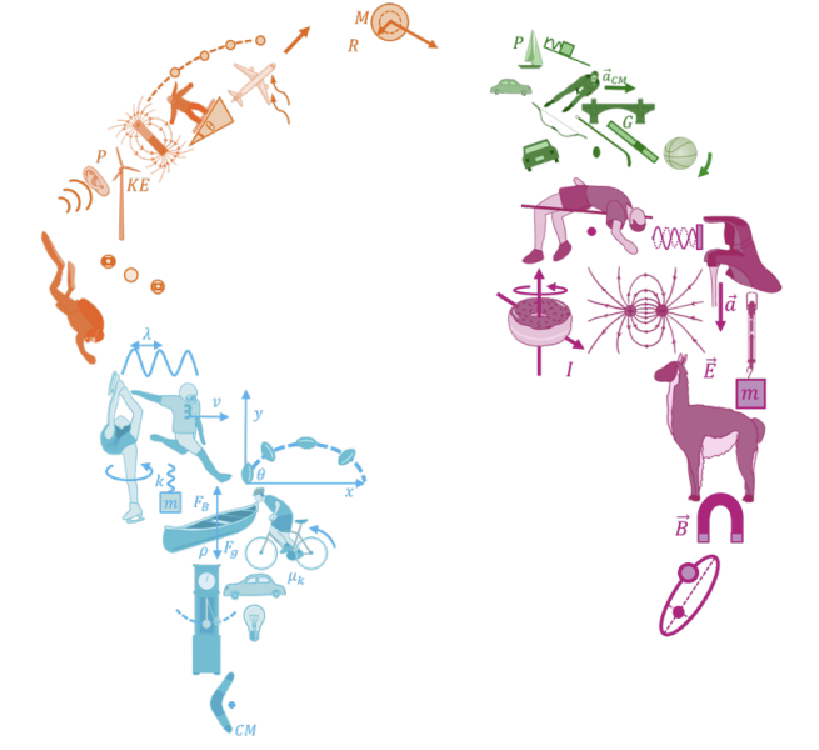
\includegraphics[width=4cm]{figures/BMDW/logo}
\end{textblock*}

\end{frame}

%%%%%%%%%%%%%TOC
\twocolframe{Outline}
  {\tableofcontents[sections={1,2}, subsectionstyle=show/show]\thispagestyle{empty}}
  {\tableofcontents[sections={3}, subsectionstyle=show/show]}
%%%%%%%%%%%%%%%%%%%%%%%%%







%%%%%%%%%%%%%%%%%%%%%%%%%%%%%%%%
\section{Faraday's Law}
\label{sec:faradayslaw}
\title{Faraday's Law}


%%%%%%%%%%%%%%%%%%%%%%%%%
\begin{frame}
\titlepage
\thispagestyle{empty}
\end{frame}

%%%%%%%%%%%%%%%%%%%%%%%




\subsection{Electromagnetism}
\label{subsec:electromagnetism}
\twocolframesf{Electromagnetism}
{
\begin{itemize}
\item So far, we have looked at static cases:
\begin{enumerate}
\item An electric field that does not change with time (e.g. created by a charge that is not moving)
\item A magnetic field that does not change with time (e.g. created by a current that is constant)
\end{enumerate}
\item<1> We have seen three of the four equations that explain all of electromagnetic phenomena
\item<2> Faraday’s law (the 4th equation) connects electric and magnetic fields
\item<2> Faraday’s law is the only one that explicitly references time
\end{itemize}
}
{
\only<1>{
\begin{align*}
\oint \vec E \cdot d\vec A &= \frac{Q^{enc}}{\epsilon_0}\\
\oint \vec B \cdot d\vec A &= 0\\
\oint \vec B \cdot d\vec l&= \mu_0 I^{enc}\\
\end{align*}
}
\only<2>{
\begin{align*}
\oint \vec E \cdot d\vec A &= \frac{Q{enc}}{\epsilon_0}\\
\oint \vec B \cdot d\vec A &= 0\\
\oint \vec B \cdot d\vec l&= \mu_0 I^{enc}\\
\oint \vec E \cdot d\vec l&= -\frac{d\Phi_B}{dt}\\
\end{align*}
Maxwell's equations (more or less...)
}

}

%%%%%%%%%%%%%%%%%%%%%%%%%%%%%%
\subsection{Formula}
\label{subsec:faradayformula}
\begin{bulletframe}{Faraday's Law}
\item The circulation of the electric field:
\begin{align*}
\oint \vec E \cdot d\vec l&= -\frac{d\Phi_B}{dt}
\end{align*}
\item This is zero, if $\frac{d\Phi_B}{dt}=0$, i.e. if $\Phi_B$  does not change with time (\textbf{statics}).
\pause
\item What is $\oint \vec E \cdot d\vec l$?
\begin{itemize}
\item Compare with the definition of electric potential difference:
\begin{align*}
\Delta V = (V_2-V_1) = -\int_{\vec r_1}^{\vec r_2}\vec E\cdot d\vec r
\end{align*}
\item $\oint \vec E \cdot d\vec l$ is the electric potential difference in going around a closed loop (ending where you started)
\item if $\Phi_B$  changes with time, then the electric field does net work when you go around a closed path $\rightarrow$ The electric force is no longer conservative!
\item Since $\Delta V$ in this case is the potential difference between two points that are the same, we (they) find it less awkward to call it emf (electromotive force).
\end{itemize}
\end{bulletframe}


%%%%%%%%%%%%%%%%%%%%%%%%%%%%%%
\subsection{EMF on a closed loop}
\label{subsec:emfonaclosedloop}
\twocolframesf{EMF on a closed loop}
{
\begin{itemize}
\item If a charge $q$ goes around the loop, it will gain energy given by:
\begin{align*}
W=q\Delta V
\end{align*}
\item If there is no way for the charge to loose energy (e.g. a resistor or air molecules), it will keep going around the circle faster and faster.
\item The loop does not need to be an actual physical wire, it can just be an arbitrarily drawn path.
\item If the loop is a wire, then the emf is like an ideal battery.
\end{itemize}
}
{
\centering
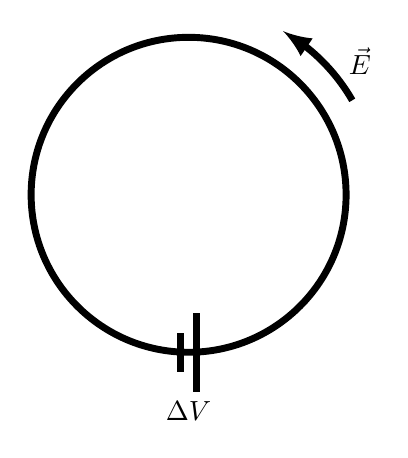
\begin{tikzpicture}[scale=1]
\tikzmath{
\R=2;
\d=0.1;
\L=0.5;
}

\draw[line width = 2.5pt] (0,0) circle(\R);
\draw[line width = 2.5pt] (\d,-\R-\L) -- (\d,-\R+\L);
\draw[line width = 2.5pt] (-\d,-\R-0.5*\L) -- (-\d,-\R+0.5*\L);

\draw[line width = 2.5pt,-latex] (30:1.2*\R) arc(30:60:1.2*\R) node[midway,right=5pt] {$\vec E$};

\node[below] at (0,-\R-\L) {$\Delta V$};
\end{tikzpicture}

}


%%%%%%%%%%%%%%%%%%%%%%%%%%%%%%
\subsection{Review: the galvonometer}
\label{subsec:reviewthegalvonometer}
\twocolframe{Review: the galvanometer}
{
\begin{itemize}
\item A coil carrying current has a magnetic dipole moment.
\item The coil wants to align its dipole moment with an external magnetic field.
\item A galvanometer is a very sensitive device for measuring current:
\begin{itemize}
\item When a current is present in the coil, the torque on the coil is proportional to current.
\item A balancing torque is provided by a restoring spring.
\end{itemize}
\end{itemize}
}
{
\capfig{0.9}{figures/Induction/galvanometer}{A galvanometer}
}



%%%%%%%%%%%%%%%%%%%%%%%%%%%%%%



%%%%%%%%%%%%%%%%%%%%%%%%%%%%%%



%%%%%%%%%%%%%%%%%%%%%%%%%%%%%%
\subsection{Induction}
\label{subsec:induction}
\twocolframe{Induction}
{
\begin{itemize}
\item Henry and Faraday both observed that currents can be induced with a magnet.
\item Faraday described it in more detail, so we refer to Faraday’s Law of Induction.
\item Currents were only induced when there was a change in the magnetic field.
\end{itemize}
}
{
\vspace{-2cm}
\capfig{1}{figures/Induction/faraday2}{Faraday's experiment showing induction between coils of wire: The liquid battery (right) provides a current which flows through the small coil (A), creating a magnetic field. When the coils are stationary, no current is induced. But when the small coil is moved in or out of the large coil (B), the magnetic flux through the large coil changes, inducing a current which is detected by the galvanometer (G). Wikipedia.}
}


%%%%%%%%%%%%%%%%%%%%%%%%%%%%%%
\begin{bulletframe}{More observations from Faraday}
\item The induced current is larger if the magnetic field is stronger.
\item The induced current is larger if the area of the loop is larger.
\item The induced current is larger if the magnet moves perpendicular to the loop.
\end{bulletframe}


%%%%%%%%%%%%%%%%%%%%%%%%%%%%%%
\subsection{Magnetic flux and Faraday's law of induction}
\label{subsec:magneticfluxandfaradayslawofinduction}
\twocolframesf{Magnetic Flux and Faraday's law of induction}
{
\begin{itemize}
\item \textbf{Magnetic flux} through area, $A$:
\begin{align*}
\Phi_B = \int \vec B \cdot d\vec A=\int BdA \cos\theta
\end{align*}
\end{itemize}
$\Delta V$ is the ``induced emf'' along the loop that bounds the area:
\begin{itemize}
\item Proportional to area of loop.
\item Proportional to magnetic field.
\item Proportional to rate of change of flux.
\item The opposite sign if $\vec B$ points in the opposite direction.
\end{itemize}
}
{
Faraday’s Law of induction:
\begin{align*}
\Delta V = -\frac{d\Phi_B}{dt}
\end{align*}
\centering

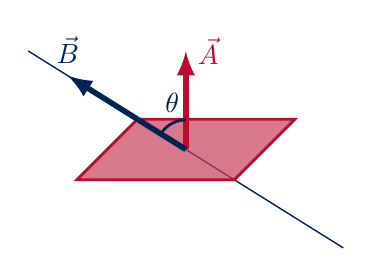
\begin{tikzpicture}[scale=0.5]
\tikzmath{
\L = 4;
\LA = 2.5;
\D=2.5;
}

\draw[color=qblue, line width =0.5] (\L,-\D,0) -- (0,0,0);

\fill[color=qred!80,opacity=0.7] (-\L/2,0,-\L/2) -- (-\L/2,0,\L/2) -- (\L/2,0,\L/2) -- (\L/2,0,-\L/2) -- cycle;
\draw[color=qred, line width = 1] (-\L/2,0,-\L/2) -- (-\L/2,0,\L/2) -- (\L/2,0,\L/2) -- (\L/2,0,-\L/2) -- cycle;

\draw[line width = 2, -latex, color=qred] (0,0,0) -- +(0,\LA,0) node[right]{$\vec A$};;
\draw[line width = 2, -latex, color=qblue] (0,0,0) -- ($(0,0,0)!0.75!(-\L,\D,0)$) node[above]{$\vec B$};;


\draw[color=qblue, line width =1] (0,0.3*\LA,0) arc (90:145:0.3*\LA) node[midway,above] {$\theta$};

\draw[color=qblue, line width =0.5] (0,0,0) -- (-\L,\D,0);


\end{tikzpicture}
\captionof*{figure}{\textit{Flux of magnetic field through an open surface. The potential difference in Faraday's Law is along the closed path that bounds the surface.}}
}



%%%%%%%%%%%%%%%%%%%%%%%%%%%%%%



%%%%%%%%%%%%%%%%%%%%%%%%%%%%%%
%%%%%%%%%%%%%%%%%%%%%%%%%%%%%%





\twocolframesf{Magnetic Flux and Faraday’s law of induction}
{
\begin{itemize}
\only<1>{\item We introduce \textbf{magnetic flux} through an area defined by a {\color{qred}loop} as:
\begin{align*}
\Phi_B = \int \vec B \cdot d\vec A=\int BdA \cos\theta
\end{align*}}
\item \textbf{Faraday’s Law} of induction:
\begin{align*}
\Delta V = -\frac{d\Phi_B}{dt}
\end{align*}
\end{itemize}
$\Delta V$ is the change in potential energy per unit charge from going around the {\color{qred}loop} once.
\only<2>{
\begin{itemize}
\item \textbf{Lenz’s Law} tells us which way the induced current goes around the loop (allowing us to ignore the minus sign):
\begin{itemize}
\item If the \textbf{flux is increasing} in the loop, then the induced current creates a magnetic field that is in the \textbf{opposite direction} of the original field.
\item If the \textbf{flux is decreasing} in the loop, then the induced current creates a magnetic field that is in the \textbf{same direction} as the original field.
\end{itemize}
\end{itemize}
}
}
{

\centering
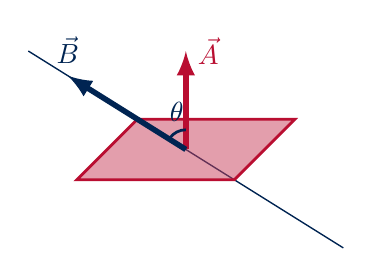
\begin{tikzpicture}[scale=0.5]
\tikzmath{
\L = 4;
\LA = 2.5;
\D=2.5;
}

\draw[color=qblue, line width =0.5] (\L,-\D,0) -- (0,0,0);

\fill[color=qred!80,opacity=0.5] (-\L/2,0,-\L/2) -- (-\L/2,0,\L/2) -- (\L/2,0,\L/2) -- (\L/2,0,-\L/2) -- cycle;
\draw[color=qred, line width = 1] (-\L/2,0,-\L/2) -- (-\L/2,0,\L/2) -- (\L/2,0,\L/2) -- (\L/2,0,-\L/2) -- cycle;

\draw[line width = 2, -latex, color=qred] (0,0,0) -- +(0,\LA,0) node[right]{$\vec A$};;
\draw[line width = 2, -latex, color=qblue] (0,0,0) -- ($(0,0,0)!0.75!(-\L,\D,0)$) node[above]{$\vec B$};;


\draw[color=qblue, line width =1] (0,0.2*\LA,0) arc (90:145:0.2*\LA) node[midway,above] {$\theta$};

\draw[color=qblue, line width =0.5] (0,0,0) -- (-\L,\D,0);


\end{tikzpicture}
\captionof*{figure}{\textit{Flux of magnetic field through a surface enclosed by a loop.}}
}



%%%%%%%%%%%%%%%%%%%%%%%%%%%%%%
\subsection{Review: magnetic moment}
\label{subsec:reviewmagneticmoment}
\twocolframesf{Review: Magnetic moment}
{
\begin{itemize}
\item An induced current creates its own magnetic field.
\item The magnetic field in the loop is aligned with the magnetic moment of the induced current in the loop:
\begin{align*}
\vec\mu=I\vec A
\end{align*}
\item The loop is like a bar magnet with magnetic moment $\vec\mu$, thus it will experience a torque that will tend to align the magnetic moment with the magnetic field that is inducing the current:
\begin{align*}
\vec\tau = \vec\mu \times \vec B
\end{align*}
\end{itemize}

}
{
\vspace{-1.5cm}
\capfig{0.4}{figures/Induction/mu}{Magnetic moment for a loop of current.}
\vspace{-0.5cm}
\capfig{0.6}{figures/Induction/hand}{Right hand rule for axial vectors.}
}


%%%%%%%%%%%%%%%%%%%%%%%%%%%%%%
\subsection{The minus sign in Farada's law}
\label{subsec:theminussigninfaradayslaw}
\begin{bulletframe}{The minus sign in Faraday's Law}
\item The sign of the flux depends on the choice that we make for the direction of $d\vec A$.
\begin{align*}
\Delta V = -\frac{d\Phi_B}{dt}=\textcolor{qred}{-}\frac{d}{dt}\int \vec B \cdot d\vec A
\end{align*}
\item This will determine the sign of $\Delta V$.
\item Clearly, it's not arbitrary: If we look at current through a loop, it will flow in a given direction (from high V to low V, in the direction of $\vec E$).
\item The minus sign is there to conserve energy!
\item \textbf{It refers to the direction of the magnetic moment of the induced current relative to the (arbitrary) choice that was made for the direction of $d\vec A$.}
\end{bulletframe}


%%%%%%%%%%%%%%%%%%%%%%%%%%%%%%
\begin{bulletframe}{The minus sign in Faraday's Law}
\item The sign of the flux depends on the choice that we make for the direction of $d\vec A$:
\begin{align*}
\Delta V = -\frac{d\Phi_B}{dt} = -\frac{d}{dt}\int \vec B \cdot d\vec A
\end{align*}
\item This will determine the sign of $\Delta V$. \textbf{The easiest is to ignore the sign and use Lenz’s Law} to figure out which way the induced current goes.
\end{bulletframe}


%%%%%%%%%%%%%%%%%%%%%%%%%%%%%%
\twocolframest{The minus sign in Faraday's Law}
{
\begin{itemize}
\item However, the sign is meaningful, consider the case with the shrinking ring in a constant field:
\begin{itemize}
\item If we choose \textbf{$d\vec A$ into the page}, then $\Phi_B$ is positive and decreasing in magnitude, so \textbf{$\frac{d\Phi_B}{dt} $ is negative}.
\item \textbf{\color{qred}$\Delta V$ is thus positive}. 
\item With Lenz’s Law, we can argue that the current is clockwise. 
\item By choosing the direction of $d\vec A$, we define what we consider to be the positive direction of current (with our right hand). \textbf{The sign of $\Delta V$ tells us whether the magnetic moment from the induced current is in the same direction as our choice of $d\vec A$ }.
\item The magnetic moment of the induced current is in the \textbf{\color{qred}same direction} as $d\vec A$ in this case.
\end{itemize}
\end{itemize}
}
{
\begin{align*}
\Aboxed{\Delta V &= -\frac{d\Phi_B}{dt}= -\frac{d}{dt}\int \vec B \cdot d\vec A}
\end{align*}
\centering
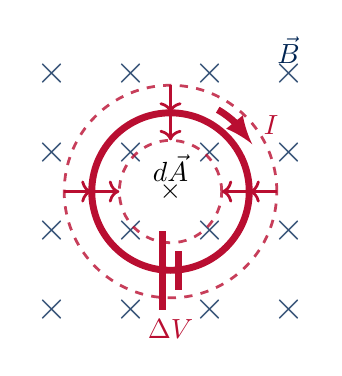
\begin{tikzpicture}[scale=1]
\tikzmath{
\R=1.;
\d=0.1;
\L=0.5;
\Nt=3;
}

\foreach \i in {0,...,\Nt}{
  \foreach \j in {0,...,\Nt}{
    \tikzmath{
      \x=-1.5*\R+\i*3*\R/\Nt;
       \y=-1.5*\R+\j*3*\R/\Nt;
    }
    \node[color=qblue!80] at (\x,\y) {\Large $\times$};
  }
}
%arrows
\draw[->,color=qred,line width = 1pt] (-1.35*\R,0) -- (-\R,0);
\draw[->,color=qred,line width = 1pt] (-\R,0) -- (-0.65*\R,0);
\draw[->,color=qred,line width = 1pt] (1.35*\R,0) -- (\R,0);
\draw[->,color=qred,line width = 1pt] (\R,0) -- (0.65*\R,0);
\draw[->,color=qred,line width = 1pt] (0,1.35*\R) -- (0,\R);
\draw[->,color=qred,line width = 1pt] (0,\R) -- (0,0.65*\R);

%circles
\draw[line width = 2.5pt,color=qred] (0,0) circle(\R);
\draw[line width = 1pt, dashed, opacity=0.8,color=qred] (0,0) circle(1.35*\R);
\draw[line width = 1pt, dashed, opacity=0.8,color=qred] (0,0) circle(0.65*\R);

%battery
\draw[line width = 2.5pt,color=qred] (-\d,-\R-\L) -- (-\d,-\R+\L);
\draw[line width = 2.5pt,color=qred] (\d,-\R-0.5*\L) -- (\d,-\R+0.5*\L);

%current and voltage
\draw[line width = 2.5pt,latex-,color=qred] (30:1.2*\R) arc(30:60:1.2*\R) node[midway,right=5pt] {$I$};
\node[below,color=qred] at (0,-\R-\L) {$\Delta V$};

\node[color=qblue,above] at (1.5*\R,1.5*\R) {$\vec B$};

\node[] at (0,0) {$\times$};
\node[above] at (0,0) {$d\vec A$};

\end{tikzpicture}
\captionof*{figure}{\textit{A shrinking loop in a magnetic field into the page will have clocwkise induced current.}}
}


%%%%%%%%%%%%%%%%%%%%%%%%%%%%%%
\twocolframest{The minus sign in Faraday's Law}
{
\begin{itemize}
\item However, the sign is meaningful, consider the case with the shrinking ring in a constant field:
\begin{itemize}
\item If we choose \textbf{$d\vec A$ out of the page}, then $\Phi_B$ is negative and increasing in value (but decreasing in magnitude), so \textbf{$\frac{d\Phi_B}{dt} $ is positive}.
\item \textbf{\color{qred}$\Delta V$ is thus negative}. 
\item With Lenz’s Law, we can argue that the current is clockwise. 
\item By choosing the direction of $d\vec A$, we define what we consider to be the positive direction of current (with our right hand). \textbf{The sign of $\Delta V$ tells us whether the magnetic moment from the induced current is in the same direction as our choice of $d\vec A$ }.
\item The magnetic moment of the induced current is in the \textbf{\color{qred}opposite} direction as $d\vec A$ in this case.
\end{itemize}
\end{itemize}
}
{
\begin{align*}
\Aboxed{\Delta V &= -\frac{d\Phi_B}{dt}= -\frac{d}{dt}\int \vec B \cdot d\vec A}
\end{align*}
\centering
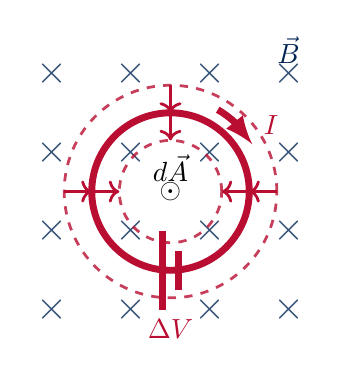
\begin{tikzpicture}[scale=1]
\tikzmath{
\R=1.;
\d=0.1;
\L=0.5;
\Nt=3;
}

\foreach \i in {0,...,\Nt}{
  \foreach \j in {0,...,\Nt}{
    \tikzmath{
      \x=-1.5*\R+\i*3*\R/\Nt;
       \y=-1.5*\R+\j*3*\R/\Nt;
    }
    \node[color=qblue!80] at (\x,\y) {\Large $\times$};
  }
}
%arrows
\draw[->,color=qred,line width = 1pt] (-1.35*\R,0) -- (-\R,0);
\draw[->,color=qred,line width = 1pt] (-\R,0) -- (-0.65*\R,0);
\draw[->,color=qred,line width = 1pt] (1.35*\R,0) -- (\R,0);
\draw[->,color=qred,line width = 1pt] (\R,0) -- (0.65*\R,0);
\draw[->,color=qred,line width = 1pt] (0,1.35*\R) -- (0,\R);
\draw[->,color=qred,line width = 1pt] (0,\R) -- (0,0.65*\R);

%circles
\draw[line width = 2.5pt,color=qred] (0,0) circle(\R);
\draw[line width = 1pt, dashed, opacity=0.8,color=qred] (0,0) circle(1.35*\R);
\draw[line width = 1pt, dashed, opacity=0.8,color=qred] (0,0) circle(0.65*\R);

%battery
\draw[line width = 2.5pt,color=qred] (-\d,-\R-\L) -- (-\d,-\R+\L);
\draw[line width = 2.5pt,color=qred] (\d,-\R-0.5*\L) -- (\d,-\R+0.5*\L);

%current and voltage
\draw[line width = 2.5pt,latex-,color=qred] (30:1.2*\R) arc(30:60:1.2*\R) node[midway,right=5pt] {$I$};
\node[below,color=qred] at (0,-\R-\L) {$\Delta V$};

\node[color=qblue,above] at (1.5*\R,1.5*\R) {$\vec B$};

\node[] at (0,0) {$\odot$};
\node[above] at (0,0) {$d\vec A$};

\end{tikzpicture}
\captionof*{figure}{\textit{A shrinking loop in a magnetic field into the page will have clocwkise induced current.}}
}

%%%%%%%%%%%%%%%%%%%%%%%%%%%%%%
\begin{bulletframe}{The minus sign in Faraday's Law}
\item Usually, can ignore and just use Lenz's Law (i.e. conservation of energy) to argue the direction of the induced current. 
\item If it's not clear, it's easiest to \textbf{pick $d\vec A$ so that $\vec B \cdot d\vec A>0$} (so that $d\vec A$ has at least a component parallel to $\vec B$).
\item Sometimes there's no choice (e.g. a rotating coil), you need to pay attention and be clear about your choice of $d\vec A$.

\end{bulletframe}

%%%%%%%%%%%%%%%%%%%%%%%%%%%%%%






%%%%%%%%%%%%%%%%%%%%%%%%%%%%%%%%
\section{Lenz's Law}
\label{sec:lenzslaw}
\title{Lenz's Law}


%%%%%%%%%%%%%%%%%%%%%%%%%
\begin{frame}
\titlepage
\thispagestyle{empty}
\end{frame}

%%%%%%%%%%%%%%%%%%%%%%%












%%%%%%%%%%%%%%%%%%%%%%%%%%%%%%%%%%%%%
\subsection{Conservation of energy to the rescue!}
\label{subsec:conservationofenergytotherescue}
\begin{bulletframe}{Conservation of energy to the rescue!}
\item The current induced in a coil will create its own magnetic field.
\begin{itemize}
\item Current in a coil creates a magnetic field, right?!
\end{itemize}
\item The total magnetic field is the ``original'' magnetic field plus the one created by the induced current.
\item[$\rightarrow$] If the magnetic field from the induced current changes the flux in a way to induce more current, then we are creating an infinite amount of current (and energy)! 
\item[$\rightarrow$] The induced current must create a magnetic field that opposes the change in flux of the original magnetic field.
\end{bulletframe}


%%%%%%%%%%%%%%%%%%%%%%%%%%%%%%%%%%%%




%%%%%%%%%%%%%%%%%%%%%%%%%%%%%%%%%%%%%7
\subsection{Theory}
\label{subsec:leztheory}
\begin{bulletframe}{Lenz's Law}
\item The induced current is in such a direction as to create a magnetic field that opposes the change in flux:
\begin{itemize}
\item If the \textbf{flux is increasing} in the loop, then the induced current creates a magnetic field that is in the \textbf{opposite direction} of the original field.
\item If the \textbf{flux is decreasing} in the loop, then the induced current creates a magnetic field that is in the \textbf{same direction} as the original field.
\end{itemize}

\end{bulletframe}

%%%%%%%%%%%%%%%%%%%%%%%%%%%%%%%%%%%%%

\twocolframe{Lenz's Law}
{
\begin{itemize}
\item The magnetic field flux above the magnet decreases if the magnet falls down.
\begin{itemize}
\item A current is induced to create a magnetic field to restore the flux
\item That magnetic field attracts the magnet!
\end{itemize}
\end{itemize}
}
{
\capfig{0.75}{figures/Induction/lenz}{\url{http://physicsbuzz.physicscentral.com/2014/09/build-your-own-time-warp-tube.html}}
}


%%%%%%%%%%%%%%%%%%%%%%%%%%%%%%


%%%%%%%%%%%%%%%%%%%%%%%%%%%%%%
\subsection{Current in a coil with N loops}
\label{subsec:currentinacoilwithnloops}
\twocolframesf{Current in a coil with N loops}
{
\begin{itemize}
\item Each loop can be considered separately (each has an induced emf from the flux changing through it).
\item Each loop is like a little battery, and the loops are all in series.
\item The (identical) emfs from each loop just add together:
\begin{align*}
\Delta V = -N \frac{d\Phi_B}{dt}
\end{align*}
where $\Phi_B$ is the flux through one loop.
\end{itemize}

}
{
\centering
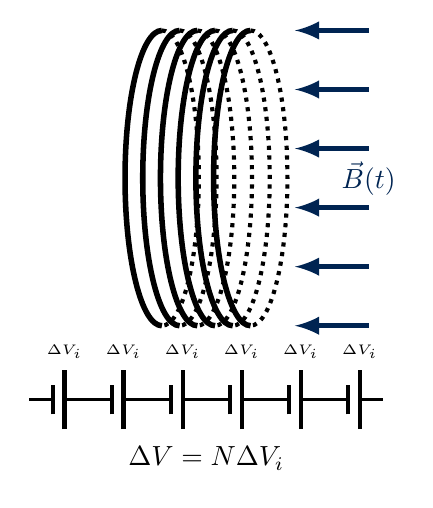
\begin{tikzpicture}[scale=0.75]

\tikzmath{
\R = 2.5;%charge radius
\f = 0.25;
\L = 1.5;
\Nt = 5;
\d=0.1;
\LV=0.5;
\LL=5;
}

%\draw[-latex] (0,0) -- (0,1.25*\R) node[left] {$y$};
%\draw[-latex] (0,0) -- (1.25*\R,0) node[below] {$x$};

\foreach \i in {0,...,\Nt}{
 \tikzmath{
 \h = -\L/2+\i*\L/\Nt;
 \hb=-\R+\i*2*\R/\Nt;
 \xl=-\LL/2+\i*\LL/\Nt;
 }
 
 %batteries
 \draw[line width = 1.5pt] (\xl+\d,-1.5*\R-\LV) -- (\xl+\d,-1.5*\R+\LV) node[above]{\tiny $\Delta V_i$ };
 \draw[line width = 1pt] (\xl+\d,-1.5*\R) -- (\xl+5*\d,-1.5*\R);
 \draw[line width = 1pt] (\xl-5*\d,-1.5*\R) -- (\xl-\d,-1.5*\R);
 \draw[line width = 1.5pt] (\xl-\d,-1.5*\R-0.5*\LV) -- (\xl-\d,-1.5*\R+0.5*\LV);
 
 %loops
 \draw[line width=2] (\h,-\R) arc(270:90:{\R*\f} and {\R});
 \draw[line width=1.5, dotted] (\h,\R) arc(90:-90:{\R*\f} and {\R});

 %mag field arrows 
 \draw[-latex, line width =2, color = qblue] (1.1*\R,\hb) -- + (-0.5*\R,0);
}

\node[color=qblue] at (1.1*\R,0) {$\vec B(t)$};
\node at (0,-1.5*\R-2*\LV) {$\Delta V = N\Delta V_i$};


\end{tikzpicture}
}


%%%%%%%%%%%%%%%%%%%%%%%%%%%%%%
\subsection{Motional emf}
\twocolframesf{Motional emf}
{
\begin{itemize}
\item Refers specifically to the case when the magnetic field is constant and the change in flux comes from motion:
\begin{align*}
\Phi_B=\int \vec B\cdot d\vec A=\int BdA\cos\theta
\end{align*}
\end{itemize}
Two options:
\begin{enumerate}
\item The angle  is changing with time (a generator).
\item The area of the loop is changing with time (the sliding bar).
\end{enumerate}

}
{
\capfig{0.7}{figures/Induction/motor}{Flux is changed by rotation.}


\centering
\begin{circuitikz}[scale=0.75]

\tikzmath{
\L=5;
\h=2;
\Nt=8;
\Lv=1;
}

%bfield
\foreach \i in {1,...,7}{
 \tikzmath{
 \x = -\L/2+\i*\L/\Nt;
 }
 \node[color=qblue!80] at (\x,0.25*\h) {\Large $\odot$};
 \node[color=qblue!80] at (\x,-0.25*\h) {\Large $\odot$};
}


\draw [color=gray, line width=5pt] (-\L/2,\h/2) -- (\L/2,\h/2);
\draw [color=gray, line width=5pt] (-\L/2,-\h/2) -- (\L/2,-\h/2);


\draw [color=black, line width=3pt] (-0.*\L,-\h/2) -- (-0.*\L,\h/2);
\draw [color=black, line width=1.5pt,-latex] (0.*\L,0) -- +(-\Lv,0) node[left]{$\vec v$};

\draw (\L/2,\h/2) [R=$R$] to (\L/2,-\h/2);
\node[color=qblue] at (0.25*\L,0) {$\vec B$};
\draw[latex-latex] (-0.55*\L, -0.5*\h) -- (-0.55*\L, 0.5*\h) node[midway,left] {$l$};


\end{circuitikz}
\captionof*{figure}{\textit{Flux is changed by change in area.}}
}


%%%%%%%%%%%%%%%%%%%%%%%%%%%%%%


%%%%%%%%%%%%%%%%%%%%%%%%%%%%%%
\subsection{A bar moving on rails}
\twocolframesf{A bar moving on rails}
{\scriptsize
\begin{itemize}
\item<1-> The area increases with time:%
\begin{align*}%
A=l(w_0+vt)%
\end{align*}%
\item<2-> The flux is ($\vec A$ out of the page):%
\begin{align*}%
\Phi_B(t)=AB=Bl(w_0+vt)%
\end{align*}%
\item<3-> The induced emf:%
\begin{align*}%
\Delta V=-\frac{d\Phi_B}{dt}=-Blv%
\end{align*}%
\item<4-> The induced current:%
\begin{align*}%
I=\frac{\Delta V}{R}=-\frac{Blv}{R}%
\end{align*}%
\only<4->{
(negative, $\vec \mu$ into the page since $\vec A$ out of the page, clockwise current)
}
\end{itemize}
}
{

\centering
\begin{circuitikz}[scale=1]

\tikzmath{
\L=4.5;
\h=2;
\Nt=8;
\Lv=1;
\xb=0;
}

%bfield
\foreach \i in {1,...,7}{
 \tikzmath{
 \x = -\L/2+\i*\L/\Nt;
 }
 \node[color=qblue!80] at (\x,0.25*\h) {\Large $\odot$};
 \node[color=qblue!80] at (\x,-0.25*\h) {\Large $\odot$};
}


\draw [color=gray, line width=5pt] (-\L/2,\h/2) -- (\L/2,\h/2);
\draw [color=gray, line width=5pt] (-\L/2,-\h/2) -- (\L/2,-\h/2);


\draw [color=black, line width=3pt] (\xb,-\h/2) -- (\xb,\h/2);
\draw [color=black, line width=1.5pt,-latex] (\xb,0) -- +(-\Lv,0) node[left]{$\vec v$};

\draw (\L/2,\h/2) [R=$R$] to (\L/2,-\h/2);
\node[color=qblue] at (0.25*\L,0) {$\vec B$};
\draw[latex-latex] (-0.55*\L, -0.5*\h) -- (-0.55*\L, 0.5*\h) node[midway,left] {$l$};
\draw[latex-latex] (0.5*\L, 0.6*\h) -- (\xb, 0.6*\h) node[midway,above] {$w(t)=w_0+vt$};


\only<5>{

\node[color=qred] at (\xb+0.2,\h/2) {$+$};
\node[color=qred] at (\xb-0.2,\h/2) {$+$};
\node[color=qred] at (\xb+0.2,0.4*\h) {$+$};
\node[color=qred] at (\xb-0.2,0.4*\h) {$+$};
\node[color=qred] at (\xb+0.2,0.3*\h) {$+$};
\node[color=qred] at (\xb-0.2,0.3*\h) {$+$};

\node[color=qred] at (\xb+0.2,-\h/2) {$-$};
\node[color=qred] at (\xb-0.2,-\h/2) {$-$};
\node[color=qred] at (\xb+0.2,-0.4*\h) {$-$};
\node[color=qred] at (\xb-0.2,-0.4*\h) {$-$};
\node[color=qred] at (\xb+0.2,-0.3*\h) {$-$};
\node[color=qred] at (\xb-0.2,-0.3*\h) {$-$};
}

\end{circuitikz}
\captionof*{figure}{\textit{A bar moving on rails.}}

\only<5->{
\vspace{-1cm}
\begin{exampleblock}{Remember the Hall Effect?}
\tiny
\begin{itemize}
\item Free charges feel a magnetic force:
\begin{align*}
F_B=qvB
\end{align*}
\item Equilibrium between the electric and magnetic forces:
\begin{align*}
qvB=qE=q\frac{\Delta V}{l} \quad \rightarrow \quad \Delta V = Blv
\end{align*}
\end{itemize}
The emf exists event if there is no closed loop or rails!
\end{exampleblock}
}


\only<5>{
\begin{tikzpicture}[remember picture,overlay]
\node at ([yshift=2cm]current page.center) {
\includegraphics[scale=0.5]{figures/Induction/member}};
\end{tikzpicture}
}
}


%%%%%%%%%%%%%%%%%%%%%%%%%%%%%%



%%%%%%%%%%%%%%%%%%%%%%%%%%%%%%
\twocolframesf{A bar moving on rails}
{\scriptsize
\begin{itemize}
\item The induced current:
\begin{align*}%
I=\frac{\Delta V}{R}=-\frac{Blv}{R}%
\end{align*}%
\item The magnitude of the magnetic force on the bar is:
\begin{align*}%
F=IlB=\frac{B^2l^2v}{R}
\end{align*}%
\item The power to move the bar is (force exerted at constant speed):
\begin{align*}%
P=Fv=\frac{B^2l^2v^2}{R}
\end{align*}%
\item The power dissipated in the resistor is:
\begin{align*}%
P=I^2R=\frac{B^2l^2v^2}{R}
\end{align*}%
\end{itemize}
}
{

\centering
\begin{circuitikz}[scale=1]

\tikzmath{
\L=4.5;
\h=2;
\Nt=8;
\Lv=1;
\xb=0;
}

%bfield
\foreach \i in {1,...,7}{
 \tikzmath{
 \x = -\L/2+\i*\L/\Nt;
 }
 \node[color=qblue!80] at (\x,0.25*\h) {\Large $\odot$};
 \node[color=qblue!80] at (\x,-0.25*\h) {\Large $\odot$};
}


\draw [color=gray, line width=5pt] (-\L/2,\h/2) -- (\L/2,\h/2);
\draw [color=gray, line width=5pt] (-\L/2,-\h/2) -- (\L/2,-\h/2);


\draw [color=black, line width=3pt] (\xb,-\h/2) -- (\xb,\h/2);
\draw [color=black, line width=1.5pt,-latex] (\xb,0) -- +(-\Lv,0) node[left]{$\vec v$};
\draw [color=qred, line width=1.5pt,-latex] (\xb,0) -- +(\Lv,0) node[right]{$\vec F$};
\draw [color=black, line width=3pt,-latex] (0,0) -- +(0,0.75) node[right]{$I$};

\draw (\L/2,\h/2) [R=$R$] to (\L/2,-\h/2);
%\node[color=qblue] at (0.25*\L,0) {$\vec B$};
\draw[latex-latex] (-0.55*\L, -0.5*\h) -- (-0.55*\L, 0.5*\h) node[midway,left] {$l$};
\draw[latex-latex] (0.5*\L, 0.6*\h) -- (\xb, 0.6*\h) node[midway,above] {$w(t)=w_0+vt$};


\end{circuitikz}
\captionof*{figure}{\textit{There is a force on the bar from the induced current}}

%\vspace{-1cm}
\begin{exampleblock}{Conservation of energy}
\scriptsize
The force has to oppose the motion, or you would get free current!\\
The rate at which work is done to pull the bar is the same as the rate at which energy is dissipated in the resistor.
\end{exampleblock}


}


%%%%%%%%%%%%%%%%%%%%%%%%%%%%%%%%%%%%%








%%%%%%%%%%%%%%%%%%%%%%%%%%%%%%%%
\section{Real World Examples}
\label{sec:realworldsexamples}
\title{Real World Examples}


%%%%%%%%%%%%%%%%%%%%%%%%%
\begin{frame}
\titlepage
\thispagestyle{empty}
\end{frame}

%%%%%%%%%%%%%%%%%%%%%%%







%%%%%%%%%%%%%%%%%%%%%%%%%%

\subsection{The generator}
\label{subsec:thegenerator}
\twocolframesf{The Generator}
{
\begin{itemize}
\item Convert mechanical work into electrical energy.
\item You have to do work (exert a torque) to keep a coil spinning in a magnetic field.
\item The work is usually done by a turbine.
\item The turbine is powered by:
\begin{itemize}
\item High pressure water from a change in height (hydro power).
\item High pressure steam created from a heat source (nuclear fission, fossil fuel burning).
\end{itemize}
\item Wind and tides can also be used to rotate a coil in a magnetic field.
\end{itemize}
}
{
\vspace{-1cm}
\capfig{0.9}{figures/Induction/turbine1}{}
\vspace{-1cm}
\capfig{0.9}{figures/Induction/turbine2}{}
}



%%%%%%%%%%%%%%%%%%%%%%%%%%%%%%




%%%%%%%%%%%%%%%%%%%%%%%%%%%%%%
\subsubsection{Modelling a generator}
\label{subsubsec:modellingagenerator}
\twocolframesf{Modelling a generator}
{
\begin{itemize}
\item<1-> We rotate a coil about the $y$ axis with an angular velocity $\vec\omega=\omega\hat y$ in a constant magnetic field, $\vec B=B\hat x$. 
\item<2-> We choose $\vec A$ to be in the $\hat x$ direction at $t=0$:
\begin{align*}
\vec A = A(\cos(\omega t)\hat x - \sin(\omega t)\hat z)
\end{align*}
\item<3-> The induced EMF is (for N loops in the coil):
\begin{align*}
\Delta V = -N \frac{d\Phi_B}{dt}= -N \frac{d}{dt}\vec A\cdot \vec B=NAB\omega\sin(\omega t)
\end{align*}
\end{itemize}
\only<3->{
\scriptsize
This leads to sinusoidal (AC) voltage. Since $\Delta V$ changes sign as a function of time, the induced current keeps changing direction (relative direction of $\vec A$ and $\vec \mu$).
}

}
{
\vspace{-1cm}
\centering
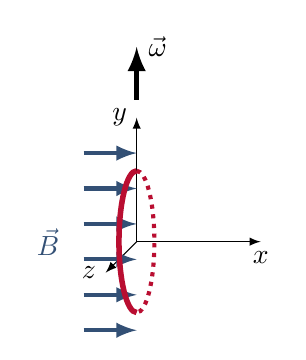
\begin{tikzpicture}[scale=0.9]
\tikzmath{
\R=1;
\f=0.25;
\Nb=5;
\LB=0.75;
}

%axes:
 \draw[-latex] (0,0) -- (1.75*\R,0) node[below]{$x$}; 
 \draw[-latex] (0,0) -- (0,1.75*\R) node[left]{$y$}; 
 \draw[-latex] (0,0) -- (-\f*1.75*\R,-\f*1.75*\R) node[left]{$z$}; 
%back of ring
 \draw[line width=1.5, dotted, color=qred] (0,\R) arc(90:-90:{\R*\f} and {\R});
%B-field
 \foreach \i in {0,...,\Nb}{
 \tikzmath{
   \h=-1.25*\R+\i*2.5*\R/\Nb;
  }
  \draw[color=qblue!80,-latex,line width = 1.5] (-\LB,\h) -- +(\LB,0);
 }
 %front of ring
 \draw[line width=2, color=qred] (0,-\R) arc(270:90:{\R*\f} and {\R});
 
 \node[color=qblue!80] at (-1.25*\R,0) {$\vec B$};
 \draw[line width=2, color=black, -latex] (0,2*\R) -- +(0,\LB) node[right] {$\vec \omega$};
\end{tikzpicture}
%\vspace{0.8cm}
\captionof*{figure}{\textit{Side view at time $t=0$.}}
%
%
\vspace{-0.2cm}
%%%%%%%%%%%%%%%%%%5top view
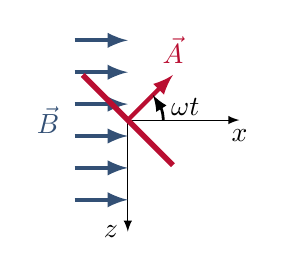
\begin{tikzpicture}[scale=0.9]
\tikzmath{
\R=0.9;
\Rsq=\R/sqrt(2);
\f=0.25;
\Nb=5;
\LB=0.75;
\Ra=0.5;
}

%axes:
 \draw[-latex] (0,0) -- (1.75*\R,0) node[below]{$x$}; 
 \draw[-latex] (0,0) -- (0,-1.75*\R) node[left]{$z$}; 

%B-field
 \foreach \i in {0,...,\Nb}{
 \tikzmath{
   \h=-1.25*\R+\i*2.5*\R/\Nb;
  }
  \draw[color=qblue!80,-latex,line width = 1.5] (-\LB,\h) -- +(\LB,0);
 }

 \draw[line width=2, color=qred] (-\Rsq,\Rsq) -- (\Rsq,-\Rsq);
 \draw[line width=1.5, color=qred,-latex] (0,0) -- (\Rsq,\Rsq) node[above]{$\vec A$};
 \draw[line width=1.,-latex] (\Ra,0) arc (0:45:\Ra) node[midway,right] {$\omega t$};
 \node[color=qblue!80] at (-1.25*\R,0) {$\vec B$};
\end{tikzpicture}
\captionof*{figure}{\textit{Top view at time $t$.}}

}



%%%%%%%%%%%%%%%%%%%%%%%%%%%%%%
\subsubsection{Magnetic moment and torque}
\label{subsubsec:magneticmomentandtorque}
\twocolframesf{Generator: magnetic moment and torque}
{\scriptsize
\begin{itemize}
\item<1-> The induced EMF is (for N loops in the coil):
\begin{align*}
\Delta V = -N \frac{d\Phi_B}{dt}= -N \frac{d}{dt}\vec A\cdot \vec B=NAB\omega\sin(\omega t)
\end{align*}
\item<2-> If the coil has resistance R:
\begin{align*}
\vec\mu&=I\vec A = \frac{\Delta V}{R}\vec A\\
&=\frac{NAB\omega}{R}\sin(\omega t)A(\cos(\omega t)\hat x - \sin(\omega t)\hat z)
\end{align*}
\item<3-> The torque on the loop from the magnetic field is thus:
\begin{align*}
\vec\tau=\vec\mu\times\vec B=\frac{NA^2B^2\omega}{R}\sin^2(\omega t)(-\hat y)
\end{align*}
\end{itemize}
\only<3->{
\vspace{-0.5cm}
\scriptsize
We must thus exert a torque in the positive y direction (same direction as angular velocity) opposite of the torque from the magnetic field to keep the coil rotating at constant speed.
}

}
{
\vspace{-1cm}
\centering
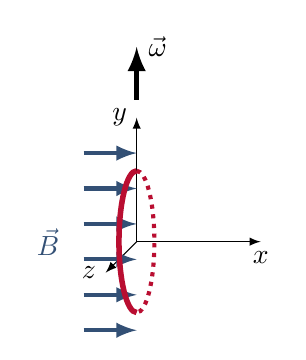
\begin{tikzpicture}[scale=0.9]
\tikzmath{
\R=1;
\f=0.25;
\Nb=5;
\LB=0.75;
}

%axes:
 \draw[-latex] (0,0) -- (1.75*\R,0) node[below]{$x$}; 
 \draw[-latex] (0,0) -- (0,1.75*\R) node[left]{$y$}; 
 \draw[-latex] (0,0) -- (-\f*1.75*\R,-\f*1.75*\R) node[left]{$z$}; 
%back of ring
 \draw[line width=1.5, dotted, color=qred] (0,\R) arc(90:-90:{\R*\f} and {\R});
%B-field
 \foreach \i in {0,...,\Nb}{
 \tikzmath{
   \h=-1.25*\R+\i*2.5*\R/\Nb;
  }
  \draw[color=qblue!80,-latex,line width = 1.5] (-\LB,\h) -- +(\LB,0);
 }
 %front of ring
 \draw[line width=2, color=qred] (0,-\R) arc(270:90:{\R*\f} and {\R});
 
 \node[color=qblue!80] at (-1.25*\R,0) {$\vec B$};
 \draw[line width=2, color=black, -latex] (0,2*\R) -- +(0,\LB) node[right] {$\vec \omega$};
\end{tikzpicture}
%\vspace{0.8cm}
\captionof*{figure}{\textit{Side view at time $t=0$.}}
%
%
\vspace{-0.2cm}
%%%%%%%%%%%%%%%%%%5top view
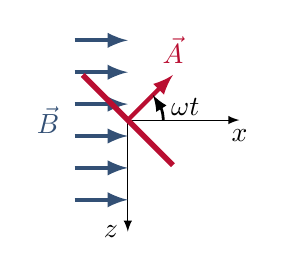
\begin{tikzpicture}[scale=0.9]
\tikzmath{
\R=0.9;
\Rsq=\R/sqrt(2);
\f=0.25;
\Nb=5;
\LB=0.75;
\Ra=0.5;
}

%axes:
 \draw[-latex] (0,0) -- (1.75*\R,0) node[below]{$x$}; 
 \draw[-latex] (0,0) -- (0,-1.75*\R) node[left]{$z$}; 

%B-field
 \foreach \i in {0,...,\Nb}{
 \tikzmath{
   \h=-1.25*\R+\i*2.5*\R/\Nb;
  }
  \draw[color=qblue!80,-latex,line width = 1.5] (-\LB,\h) -- +(\LB,0);
 }

 \draw[line width=2, color=qred] (-\Rsq,\Rsq) -- (\Rsq,-\Rsq);
 \draw[line width=1.5, color=qred,-latex] (0,0) -- (\Rsq,\Rsq) node[above]{$\vec A$};
 \draw[line width=1.,-latex] (\Ra,0) arc (0:45:\Ra) node[midway,right] {$\omega t$};
 \node[color=qblue!80] at (-1.25*\R,0) {$\vec B$};
\end{tikzpicture}
\captionof*{figure}{\textit{Top view at time $t$.}}

}


%%%%%%%%%%%%%%%%%%%%%%%%%%%%%%
\subsubsection{Generator or motor?}
\label{subsubsec:generatorormotor}
\twocolframesf{Generator or Motor?}
{
\begin{itemize}
\item If we do mechanical work, we can rotate a coil in a magnetic field and induce a current:
\begin{itemize}
\item Mechanical energy $\rightarrow$ Electrical energy
\end{itemize}
\item If we instead apply a voltage to drive a current in the coil, the coil starts to rotate (an electric motor)
\begin{itemize}
\item Electrical energy $\rightarrow$ Mechanical energy
\end{itemize}
\item So what about the bar on rails? If we pull on the bar, we can induce a current. What if we instead apply a voltage? What happens? What’s that called?\only<2>{ A railgun...}
\end{itemize}
}
{
\only<1>{
\begin{columns}
\column{0.5\textwidth}
\capfig{0.9}{figures/Induction/turbine1}{A turbine.}
\column{0.5\textwidth}
\capfig{0.9}{figures/Induction/motor2-0}{A motor.}
%\animategraphics[loop,width=0.9\textwidth]{10}{figures/motor2-}{0}{2}
\end{columns}
\capfig{0.9}{figures/Induction/bar}{A bar on rails.}
}


\only<2>{
\begin{columns}
\column{0.5\textwidth}
\capfig{1.}{figures/Induction/railgun1}{}
\column{0.5\textwidth}
\capfig{1.}{figures/Induction/railgun2}{}
\end{columns}
\vspace{-1cm}
\capfig{0.75}{figures/Induction/railgun3}{To add to the stupid things physicists have invented...}
}

}


%%%%%%%%%%%%%%%%%%%%%%%%%%%%%%
\subsection{The induced electric field}
\label{subsec:theinducedelectricfield}
\begin{bulletframe}{The induced electric field}
\item Faraday’s original formulation was in terms of induced voltage:
\begin{align*}
\Delta V = -\frac{d\Phi_B}{dt}
\end{align*}
\item But we can think of this in terms of induced electric field:
\begin{align*}
\oint \vec E\cdot d\vec l = -\frac{d\Phi_B}{dt}
\end{align*}
since, after all, voltage is just (negative) work done per unit charge by an electric field.
\end{bulletframe}




%%%%%%%%%%%%%%%%%%%%%%%%%%%%%%
\begin{bulletframe}{The induced electric field}
\item If we want to be able to calculate an electric field from:
\begin{align*}
\oint \vec E\cdot d\vec l
\end{align*}
Then, it’s easier if the integral is easy…
\item[$\rightarrow$] High degree of symmetry:
\begin{itemize}
\item $\vec E$ constant magnitude around the loop.
\item $\vec E$ and $d\vec l$ make a constant angle between them.
\end{itemize}
\item Same constraints as for Ampère’s Law!
\end{bulletframe}


%%%%%%%%%%%%%%%%%%%%%%%%%%%%%%
\twocolframesf{The induced electric field}
{
\begin{itemize}
\item Consider the uniform magnetic field inside of a solenoid. Assume that current is changing, so that magnetic field changes magnitude.
\item<2-> By symmetry, we expect the electric field to make concentric circles that are coaxial with the solenoid
\item<3> Choose a loop over which to calculate the circulation and flux:.
\begin{align*}
\oint \vec E\cdot d\vec l &=E(2\pi r)= -\frac{d\Phi_B}{dt}\\
\therefore E&=\frac{-1}{2\pi r}\frac{d\Phi_B}{dt}
\end{align*}
\end{itemize}
}
{
\centering
\begin{tikzpicture}[scale=1.0]
\tikzmath{
\R=3;
\r=0.6*\R;
\Nb=11;
\LB=1;
}


 \draw[line width=1.5] (0,0) circle(\R);
%B-field
\begin{scope}
\clip (0,0) circle(\R);
 \foreach \i in {0,...,\Nb}{
 \foreach \j in {0,...,\Nb}{
 \tikzmath{
   \x=-\R+\i*2*\R/\Nb;
   \y=-\R+\j*2*\R/\Nb;
  }
  \node[color=qblue!80] at (\x,\y) {\Large $\odot$};
 }}
 \end{scope}

\node[color=qblue!80, right=6pt] at (135:\R) {$\vec B$};
\draw[color=qred,line width = 2, -latex] (80:\R) arc (80:110:\R) node[midway,above] {$I$};

\only<2->{
\draw[color=qred, line width=1,-latex] (\r,0) -- +(0,\LB) node[right]{$\vec E$};
\draw[color=qred, line width=1,-latex] (-\r,0) -- +(0,-\LB) node[left]{$\vec E$};
\draw[color=qred, line width=1,-latex] (0,\r) -- +(-\LB,0) node[above]{$\vec E$};
\draw[color=qred, line width=1,-latex] (0,-\r) -- +(\LB,0) node[below]{$\vec E$};
}

\only<3>{
\draw[color=qred, line width=1] (0,0) circle(\r);
\draw[color=qred, line width=1] (0,0) -- (45:\r) node[midway,below] {$r$};

}

\end{tikzpicture}
\captionof*{figure}{\textit{A time varying magnetic field induces an electric field.}}
}


%%%%%%%%%%%%%%%%%%%%%%%%%%%%%%




%%%%%%%%%%%%%%%%%%%%%%%%%%%%%%
\subsection{Magnetic braking}
\twocolframesf{Magnetic braking}
{
\begin{itemize}
\item In the part entering the magnetic field, magnetic flux is increasing so a current is induced to create a magnetic field in the opposite direction.
\item In the part exiting the magnetic field,, the magnetic flux is decreasing, so a current is induced to create a magnetic field in the same direction.
\item At the middle, the currents from all loops go in the same direction, the force on those currents slow the disk down!
\end{itemize}
}
{
\vspace{-1cm}
\capfig{0.75}{figures/Induction/mbrake}{Magnetic brake.}
\vspace{-1cm}
\capfig{0.75}{figures/Induction/magneticbrake}{Magnetic brake (note that the field is in the opposite direction compared to above!). }
}


%%%%%%%%%%%%%%%%%%%%%%%%%%%%%%



%%%%%%%%%%%%%%%%%%%%%%%%%%%%%%
\subsection{Transformers}
\label{subsec:transformers}
\twocolframesf{Transformers}
{
\begin{itemize}
\item Used to change voltage.
\item Input coil generates changing magnetic flux (AC current).
\item Changing magnetic flux induces current (voltage) on output coil:
\begin{align*}
\Delta V_p &= -N_p\frac{d\Phi_B}{dt}\\
\Delta V_s &= -N_s\frac{d\Phi_B}{dt}\\
\therefore \frac{\Delta V_s}{\Delta V_p}=\frac{N_s}{N_p} \;\;&\rightarrow\;\; \Delta V_s=\frac{N_s}{N_p}\Delta V_p
\end{align*}
\end{itemize}
}
{
\vspace{-1cm}
\capfig{0.7}{figures/Induction/transformer}{A transformer.}
\vspace{-1cm}
\capfig{0.7}{figures/Induction/transpic}{\url{https://en.wikipedia.org/wiki/Transformer}}
}


%%%%%%%%%%%%%%%%%%%%%%%%%%%%%%



%%%%%%%%%%%%%%%%%%%%%%%%%%%%%%
\subsection{Power lines}
\label{subsec:powerlines}
\twocolframest{Power lines}
{\scriptsize
\begin{itemize}
\item Suppose that we wish to transmit 120kW through power lines with a resistance of $R=\SI{0.4}{\Omega}$. How much power do we loose in the lines?
\item We don't know the resistance of the load (the town), but we know how much power is going through the lines (the power from the plant is used in the lines and in the town), we can thus find the current:
\begin{align*}
P_{plant}=I\Delta V\;\;\rightarrow\;\; I=\frac{P_{plant}}{\Delta V}
\end{align*}
\item The power dissipated in the lines is:
\begin{align*}
P_{line}=I^2R_{line}=\frac{P^2_{plant}}{\Delta V^2}R_{line}
\end{align*}
\item If we transmit the power at \SI{240}{V}, $P_{line}=\SI{100}{kW}$ (more than 80\% loss)
\item If we transmit the power at \SI{24000}{V}, $P_{line}=\SI{10}{W}$  (much less than 1\% loss)
\end{itemize}
}
{
\capfig{0.7}{figures/Induction/powerplant}{A power plant connected to a city.}
}



%%%%%%%%%%%%%%%%%%%%%%%%%%%%%%
\subsection{Electric motor and EMF}
\label{subsec:electricmotorandemf}
\begin{bulletframe}{Electric motor and EMF}
\item Recall the electric motor:
\begin{itemize}
\item By running a current through a coil in a magnetic field, we could make the coil rotate
\item But now, we have a coil rotating in a magnetic field, so there must be an induced current in it, in addition to the current that we put in!
\end{itemize}
\end{bulletframe}




%%%%%%%%%%%%%%%%%%%%%%%%%%%%%%
\subsection{Effects of back EMF}
\label{subsec:effectsofbackemf}
\twocolframest{Back EMF}
{\scriptsize
\begin{itemize}
\item In order to conserve energy, the induced current is in the opposite direction of the current driving the motor.
\item The motor acts like a battery trying to oppose current coming in $\rightarrow$ ``back emf''.
\item When you first turn the motor on, no back emf, large current through the motor.
\item As the motor spins up, the back emf grows and the current decreases.
\item If there is no load on the motor, the back emf grows until it is just less than the driving emf (when it reaches the driving emf, the current is zero, the motor slows, the back emf goes down, the current goes back up $\rightarrow$ an equilibrium is reached).
\item In practice there is always a load from friction.
\item With no back emf, the motor would spin infinitely fast.
\end{itemize}
}
{
\capfig{0.7}{figures/Induction/backemf}{The back emf from a spinning motor acts like a battery that opposes current in a circuit. As the motor comes to speed, the back emf grows until an equlibrium is reached.}
}

%%%%%%%%%%%%%%%%%%%%%%%%%%%%%%
\begin{bulletframe}{Effects of back EMF}
\item If there is a load on the motor, it cannot spin as fast, back emf goes down, current goes up:
\begin{itemize}
\item If the current is higher, the motor can do more mechanical work ($I^2R$).
\item If the load is too high, the current could be too high in the motor and overheat it and melt it (try blocking the air intake of your hair dryer).
\end{itemize}
\item When the motor first turns on, it draws the most current:
\begin{itemize}
\item When the motor in your fridge turns on, the lights in your house momentarily dim.
\item This is because the large current draw results in an appreciable voltage drop across the resistance of the electrical wires in your house.
\item Everything in the circuit gets less voltage until the motor spins up and its current goes back down.
\end{itemize}
\end{bulletframe}


%%%%%%%%%%%%%%%%%%%%%%%%%%%%%%
\begin{frame}{Effects of back EMF}
\begin{columns}[T]
%%
\scriptsize
\column{0.33\textwidth}
\centering
\begin{circuitikz}
\tikzmath{
\L=1.5;
\h=2.5;
}
\node[draw=black] (M) at (\L/2,\h) {Motor};
\draw (0,0) [short] to (0,\h/2) [nos] to (0,\h) [short] to (M.west); 
\draw (M.east) [short] to (\L,\h) [short] to (\L,0) to [battery1] (0,0); 
\draw (0,\h/2) [voltmeter,o-o] to (\L,\h/2);
\end{circuitikz}
\\
\textbf{Switch open (motor off)}
\begin{itemize}
\item No current through motor.
\item {\color{qred} Voltmeter (high resistance) measures battery voltage.}
\item Your lights see the same voltage as the voltmeter, they are brightest.
\end{itemize}
%%
\column{0.33\textwidth}
\centering
\begin{circuitikz}
\tikzmath{
\L=1.5;
\h=2.5;
}
\node[draw=black] (M) at (\L/2,\h) {Motor};
\draw (0,0) [short] to (0,\h) [short] to (M.west); 
\draw (M.east) [short] to (\L,\h) [short] to (\L,0) to [battery1] (0,0); 
\draw (0,\h/2) [voltmeter,o-o] to (\L,\h/2);
\end{circuitikz}
\\
\textbf{Switch closed (motor accelerating)}
\begin{itemize}
\item High current through motor (low resistance).
\item {\color{qred} Voltmeter measures low voltage, since most current bypasses.}
\item Your lights see the same voltage as the voltmeter, they are dim.
\end{itemize}
%%
\column{0.33\textwidth}
\centering
\begin{circuitikz}
\tikzmath{
\L=1.5;
\h=2.5;
}
\node[draw=black] (M) at (0.35*\L,\h) {Motor};
\draw (\L,0) [battery1] to (0,0) [short] to (0,\h) [short] to (M.west); 
\draw (M.east) [battery1,invert] to (\L,\h) [short] to (\L,0); 
\draw (0,\h/2) [voltmeter,o-o] to (\L,\h/2);
\end{circuitikz}
\\
\textbf{Switch closed (motor spinning)}
\begin{itemize}
\item Back emf from the motor reduces current in the motor.
\item {\color{qred} Voltmeter goes back up to battery voltage minus back emf voltage.}
\item Your lights almost as bright as before.
\end{itemize}
\end{columns}
\end{frame}


%%%%%%%%%%%%%%%%%%%%%%%%%%%





%%%%%%%%%%%%%%%%%%%%%%%%%





%%%%%%%%%%%%%%%%%%%%%%%%%





%%%%%%%%%%%%%%%%%%%%%%%%%





%%%%%%%%%%%%%%%%%%%%%%%%





%%%%%%%%%%%%%%%%%%%%%%%%





%%%%%%%%%%%%%%%%%%%%%%%%%%%

\end{document}

